
\documentclass[14pt, a4paper]{article}
\usepackage{minitoc}
\usepackage[left=3.00cm, right=2.5cm, top=2.00cm, bottom=2.00cm]{geometry}
\usepackage{amsmath}
\usepackage{amssymb}
\usepackage{amsthm}
\usepackage{thmtools}
\usepackage{mathtools}
\usepackage{graphicx}
%\usepackage{algpseudocode}
%\usepackage{algorithm}
\usepackage[ruled,vlined,linesnumbered,algosection]{algorithm2e}
\usepackage{blindtext}
\usepackage{setspace}
\usepackage[utf8]{inputenc}
\usepackage[utf8]{vietnam}
\usepackage[center]{caption}
\usepackage[shortlabels]{enumitem}
\usepackage{fancyhdr} % header, footer
\usepackage{hyperref} % loại bỏ border với mục lục và công thức
\usepackage[nonumberlist, nopostdot, nogroupskip]{glossaries}
\usepackage{glossary-superragged}
\usepackage{tikz,tkz-tab}
\setglossarystyle{superraggedheaderborder}
\pagestyle{fancy}
%\usepackage[style=numeric,sortcites]{biblatex}
%\addbibresource{ref.bib}
%\usepackage[numbers]{natbib}
\usepackage{indentfirst}
\usepackage{multirow}
\usepackage[natbib,backend=biber,style=ieee, sorting=ynt]{biblatex}
\bibliography{ref.bib}

\usepackage{caption}
\usepackage{subcaption}

\graphicspath{{./figures/}}


\makenoidxglossaries

% Danh mục thuật ngữ

\hypersetup{
    colorlinks=false,
    pdfborder={0 0 0},
}


\fancyhf{}
\rhead{\textbf{Môn học: Một số vấn đề về đồ họa máy tính}}
\lhead{\textbf{GVHD: TS. Nguyễn Thị Bích Thủy}}
\rfoot{\thepage}
\lfoot{\textbf{Học viên thực hiện: Nguyễn Chí Thanh - 21007925}}
\renewcommand{\headrulewidth}{0.4pt}
\renewcommand{\footrulewidth}{0.4pt}


\numberwithin{equation}{section}
\numberwithin{figure}{section}

\setlength{\parindent}{0.5cm}

\setcounter{secnumdepth}{3} % Cho phép subsubsection trong report
\setcounter{tocdepth}{3} % Chèn subsubsection vào bảng mục lục

\newtheorem{dl}{Định lý}
\newtheorem{md}{Mệnh đề}
\newtheorem{bd}{Bổ đề}
\newtheorem{dn}{Định nghĩa}
\newtheorem{hq}{Hệ quả}

\numberwithin{dl}{section}
\numberwithin{md}{section}
\numberwithin{bd}{section}
\numberwithin{dn}{section}
\numberwithin{hq}{section}

\doublespacing
\AtBeginEnvironment{tabular}{\doublespacing}


\begin{document}
    \begin{titlepage}

        \newcommand{\HRule}{\rule{\linewidth}{0.5mm}} % Defines a new command for the horizontal lines, change thickness here

        \center % Center everything on the page

        %----------------------------------------------------------------------------------------
        %	HEADING SECTIONS
        %----------------------------------------------------------------------------------------
        \textsc{\LARGE Đại học Quốc Gia Hà Nội}\\[0.5cm]
        \textsc{\LARGE Trường đại học Khoa học tự nhiên}\\[0.5cm] % Name of your university/college
        \textsc{\LARGE Khoa Toán - Cơ - Tin học}\\[0.5cm]

        
\includegraphics[scale=0.2]{HUS-logo.jpg}\\[0.5cm]

        \textsc{\Large Chuyên ngành: Khoa học dữ liệu}\\[0.5cm] % Major heading such as course name


        %----------------------------------------------------------------------------------------
        %	TITLE SECTION
        %----------------------------------------------------------------------------------------

        \HRule \\[0.4cm]
        { \huge \bfseries BÀI TẬP MÔN HỌC}\\[0.4cm] % Title of your document
        \HRule \\[1.5cm]

        \textsc{\Large Môn học: Một số vấn đề về đồ họa máy tính}\\[1cm] % Minor heading such as course title


        \textsc{\Large Đề tài: Phân tích dữ liệu cuộc bầu cử \\ Tổng thống Mỹ năm 2020}\\[2cm]


        %----------------------------------------------------------------------------------------
        %	AUTHOR SECTION
        %----------------------------------------------------------------------------------------
        \begin{minipage}{0.4\textwidth}
            \begin{flushleft} \large
            \emph{Giảng viên hướng dẫn:} \\
            TS. Nguyễn Thị Bích Thủy % Supervisor's Name
            \end{flushleft}
        \end{minipage}\\[0.5cm]

        \begin{minipage}{0.4\textwidth}
        \begin{flushleft} \large
        \emph{Học viên thực hiện:}\\
        Nguyễn Chí Thanh \\
        MSHV: 21007925 \\ % Your name
        Lớp: Khoa học dữ liệu - K4
        \end{flushleft}
        \end{minipage}


        % If you don't want a supervisor, uncomment the two lines below and remove the section above
        %\Large \emph{Author:}\\
        %John \textsc{Smith}\\[3cm] % Your name

        %----------------------------------------------------------------------------------------
        %	DATE SECTION
        %----------------------------------------------------------------------------------------

        % I don't want day because it is English
        % {\large \today}\\[2cm] % Date, change the \today to a set date if you want to be precise

        %----------------------------------------------------------------------------------------
        %	LOGO SECTION
        %----------------------------------------------------------------------------------------

        %\includegraphics{logo/rsz_3logo-khtn.png}\\[1cm] % Include a department/university logo - this will require the graphicx package

        %----------------------------------------------------------------------------------------

        \vfill % Fill the rest of the page with whitespace

    \end{titlepage}

    \cleardoublepage
    \pagenumbering{gobble}
    \tableofcontents
    \newpage
    \listoffigures
    \newpage
    \glsaddall 
    \renewcommand*{\glossaryname}{Danh mục các từ viết tắt}
    \renewcommand*{\acronymname}{Danh sách từ viết tắt}
    \renewcommand*{\entryname}{Viết tắt}
    \renewcommand*{\descriptionname}{Viết đầy đủ}
    \printnoidxglossary
    \cleardoublepage
    \pagenumbering{arabic}

    %\maketitle

    \newpage

    \nocite{*}

    \begin{center}
    \section*{LỜI MỞ ĐẦU}
    \end{center}
    \addcontentsline{toc}{section}{{\bf LỜI MỞ ĐẦU}\rm}


    \newpage

    \section{Tổng quan về cuộc bầu cử tổng thống Mỹ năm 2020}

    \subsection{Diễn biến chính của cuộc bầu cử}

    Cuộc bầu cử tổng thống Hoa Kỳ năm 2020 là cuộc bầu cử tổng thống lần thứ 59, được tổ chức vào Thứ Ba, ngày 3 tháng 11 năm 2020. Lá phiếu của đảng Dân chủ thuộc về cựu phó tổng thống Joe Biden và hạ nghị sĩ Hoa Kỳ đến từ California Kamala Harris đã đánh bại tổng thống đương nhiệm của đảng Cộng hòa Donald Trump và phó tổng thống đương nhiệm Mike Pence. 
    Cuộc bầu cử diễn ra trong bối cảnh đại dịch COVID-19 toàn cầu và suy thoái kinh tế. 
    Đây là cuộc bầu cử đầu tiên kể từ năm 1992 mà tổng thống đương nhiệm không giành được nhiệm kỳ thứ hai. 
    Cuộc bầu cử chứng kiến tỷ lệ cử tri đi bầu cao nhất tính theo tỷ lệ phần trăm kể từ năm 1900, với mỗi ứng cử viên trong số hai ứng cử viên chính nhận được hơn 74 triệu phiếu bầu, vượt qua kỷ lục 69,5 triệu phiếu bầu của Barack Obama từ năm 2008. 
    Biden nhận được hơn 81 triệu phiếu bầu, số phiếu bầu nhiều nhất từng bầu cho một ứng cử viên trong cuộc bầu cử tổng thống Hoa Kỳ.

    Trong một cuộc bầu cử sơ bộ mang tính cạnh tranh có nhiều ứng cử viên nhất cho bất kỳ đảng chính trị nào trong kỷ nguyên hiện đại của nền chính trị Hoa Kỳ, Joe Biden đã giành được đề cử tổng thống của đảng Dân chủ trước đối thủ gần nhất của mình, Thượng nghị sĩ Bernie Sanders. 
    Người bạn tranh cử của Joe Biden, Kamala Harris, đã trở thành ứng cử viên phó tổng thống người Mỹ gốc Phi đầu tiên, người Mỹ gốc Á đầu tiên và là phụ nữ thứ ba giành chiến thắng trong một đảng lớn. 
    Trump giành được sự tái đề cử, nhận được tổng cộng 2.549 đại biểu, một trong những con số nhiều nhất trong lịch sử cuộc chạy đua sơ bộ tranh cử tổng thống, so với người về nhì là Bill Weld, một đại biểu trong các cuộc bầu cử sơ bộ của Đảng Cộng hòa. 
    Jo Jorgensen đã giành được đề cử tổng thống Đảng Tự do với Spike Cohen là người bạn tranh cử của Jorgensen và Howie Hawkins đã giành được đề cử tổng thống Đảng Xanh với Angela Nicole Walker là người bạn tranh cử của Hawkins.

    Các vấn đề trọng tâm của cuộc bầu cử bao gồm các tác động kinh tế và sức khỏe cộng đồng khi đại dịch COVID-19 đang diễn ra, tình trạng bất ổn trước vụ cảnh sát sát hại George Floyd.
    Tương lai của Đạo luật điều chỉnh giá cả hợp lý. Do đại dịch đang diễn ra, số lượng phiếu bầu đã được bỏ sớm và qua đường bưu điện ở mức kỷ lục. 
    Nhiều đảng viên Đảng Dân chủ đã đăng ký bỏ phiếu qua thư hơn những đảng viên Đảng Cộng hòa. 
    Do có một số lượng lớn các lá phiếu gửi qua thư, một số bang đã gặp phải sự chậm trễ trong việc kiểm phiếu và báo cáo,
    điều này dẫn đến việc các hãng tin lớn trì hoãn dự đoán Biden và Harris là tổng thống đắc cử và phó tổng thống đắc cử cho đến sáng ngày 7 tháng 11, ba ngày sau cuộc bầu cử. 
    Các hãng truyền thông lớn dự đoán một ứng cử viên giành chiến thắng trên một tiểu bang khi một tỷ lệ lớn của phiếu đã được kiểm và ứng cử viên đó đang có tỷ lệ phiếu áp đảo so với các ứng cử viên còn lại.

    Cuối cùng, ông Biden đã giành được đa số trong Đại cử tri đoàn với 306 phiếu đại cử tri, trong khi ông Trump nhận được 232. 
    Quyết định dẫn đến chiến thắng của Biden là chiến thắng của ông ở các bang Great Lakes nghiêng về đảng Dân chủ là Michigan, Pennsylvania và Wisconsin, những bang mà Trump đã giành được vào năm 2016 và cộng lại 46 phiếu đại cử tri là đủ để xoay chuyển cuộc bầu cử cho một trong hai ứng cử viên. 
    Biden cũng trở thành đảng viên Đảng Dân chủ đầu tiên giành chiến thắng trong cuộc bầu cử tổng thống ở Georgia kể từ năm 1992, ở Arizona từ năm 1996 và ở khu vực bầu cử số 2 của Nebraska kể từ năm 2008.

    Trước, trong và sau Ngày bầu cử, Trump và nhiều đảng viên Cộng hòa khác đã cố gắng lật tẩy cuộc bầu cử và lật ngược kết quả, cáo buộc sai sự thật về hành vi gian lận cử tri phổ thông và cố gắng tác động đến quá trình kiểm phiếu ở các bang. 
    Tổng đốc William Barr và các quan chức ở mỗi bang trong số 50 bang không tìm thấy bằng chứng nào về gian lận phiếu phổ phổ thông hoặc những bất thường trong cuộc bầu cử. 
    Các cơ quan liên bang giám sát an ninh bầu cử cho biết đây là cuộc bầu cử an toàn nhất trong lịch sử nước Mỹ. 
    Chiến dịch tranh cử của Trump và các đảng viên đảng Cộng hòa, bao gồm cả các thành viên Quốc hội của Đảng Cộng hòa, tiếp tục tham gia vào nhiều nỗ lực nhằm lật ngược kết quả bầu cử bằng cách đệ trình 63 vụ kiện ở một số bang (nhưng tất cả đều bị rút lại hoặc bác bỏ), 
    Các đảng viên đảng Cộng hòa cố gắng tuyên truyền các thuyết âm mưu cáo buộc gian lận để gây sức ép với các quan chức bầu cử cấp bang của Đảng Cộng hòa (đáng chú ý là Ngoại trưởng Georgia Brad Raffensperger, trong một cuộc điện thoại mà sau này được công bố rộng rãi) và các nhà lập pháp để thay đổi kết quả.
    Ngoài ra các đảng viên đảng Cộng hòa gây áp lực buộc Bộ Tư pháp tuyên bố cuộc bầu cử là "có gian lận" và cần phải được can thiệp, phản đối chứng nhận Đại Cử tri đoàn tại Quốc hội và từ chối hợp tác với quá trình chuyển giao tổng thống của Joe Biden. 
    Vụ viện lên đến đỉnh điểm khi một đám đông những người ủng hộ Trump tấn công Điện Capitol của Hoa Kỳ vào ngày 6 tháng 1 năm 2021, sau khi ông Trump liên tục nói rằng ông sẽ không bao giờ thừa nhận kết quả cuộc bầu cử. 
    Vào ngày 7 tháng 1, ông Trump thừa nhận chính quyền sắp tới mà không nhắc đến tên của Biden.
    Ông Biden và Harris được nhậm chức vào ngày 20 tháng 1 năm 2021.

    \subsection{Các ứng cử viên tranh cử tổng thống của từng Đảng}

    \subsection{Đảng Dân chủ}

    Joe Biden trở thành ứng cử viên giả định của Đảng Dân chủ vào ngày 5 tháng 6 năm 2020, khi ông có đủ số đại biểu để đảm bảo được đề cử tại đại hội toàn quốc. 
    Ông chính thức được đề cử tại hội nghị vào ngày 18 tháng 8 cùng năm.

    \begin{figure}[h!]
        \centering
        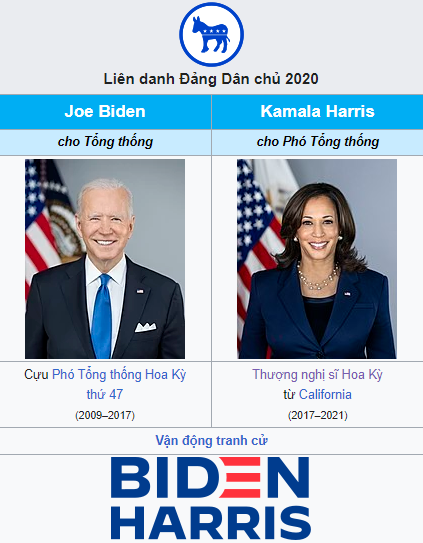
\includegraphics[width=0.6\textwidth]{Dem_Candidates.png}
        \caption{Ứng cử viên Tổng thống và ứng cử viên Phó Tổng thống Đảng Dân chủ}
    \end{figure}

    \subsection{Đảng Cộng hòa}

    Donald Trump và người bạn tranh cử Phó Tổng thống của ông, Mike Pence, đã có thể dễ dàng giành được đề cử sau khi nhận đủ số phiếu đại biểu trong cuộc bầu cử sơ bộ tổng thống của Đảng Cộng hòa năm 2020.

    \begin{figure}[h!]
        \centering
        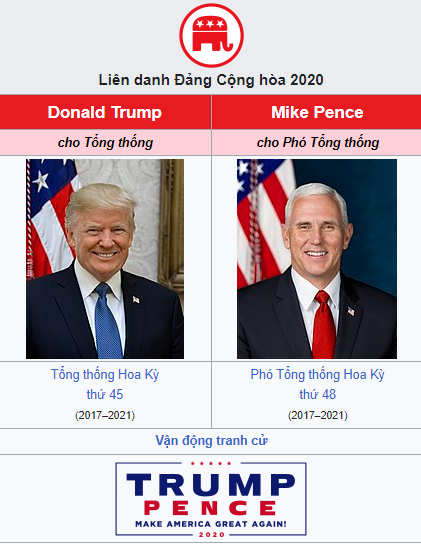
\includegraphics[width=0.6\textwidth]{Rep_Candidates.png}
        \caption{Ứng cử viên Tổng thống và ứng cử viên Phó Tổng thống Đảng Cộng hòa}
    \end{figure}

    \subsection{Đảng Tự do}

    Jo Jorgensen, người cùng tranh cử với Harry Browne vào năm 1996, đã nhận được đề cử của Đảng Tự do tại đại hội toàn quốc vào ngày 23 tháng 5 năm 2020.
    Bà đã đạt được quyền tiếp cận lá phiếu ở tất cả 50 tiểu bang và Quận Columbia.

    Mặc dù Đảng Tự do thường không giành chiến thắng trong cuộc bầu cử, nhưng có thể tác động đến kết quả của một cuộc chạy đua bằng cách lấy đi phiếu bầu của một trong các ứng cử viên của đảng chính. 
    Tuy nhiên, trong cuộc Bầu cử Tổng thống Hoa Kỳ năm 2020, Jo Jorgensen chỉ nhận được 1,1\% số phiếu phổ thông, không đủ để tác động đáng kể đến kết quả của cuộc bầu cử.

    \begin{figure}[h!]
        \centering
        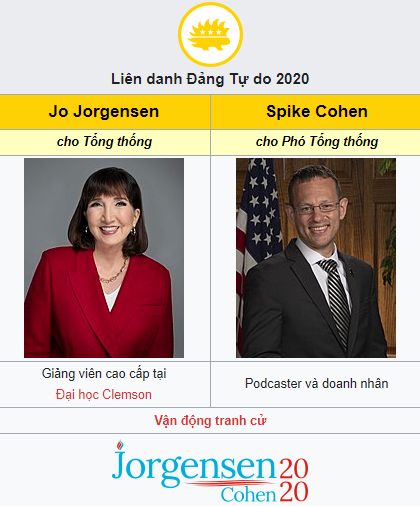
\includegraphics[width=0.6\textwidth]{Lib_Candidates.png}
        \caption{Ứng cử viên Tổng thống và ứng cử viên Phó Tổng thống Đảng Tự do}
    \end{figure}

    \subsection{Đảng Xanh}

    Howie Hawkins trở thành ứng cử viên giả định của Đảng Xanh vào ngày 21 tháng 6 năm 2020 và được đảng chính thức đề cử vào ngày 11 tháng 7 năm 2020.
    Tuy nhiên, Howie Hawkins nhận được số phiếu khá nhỏ và không có tác động đáng kể đến kết quả bầu cử. 
    Hai đảng lớn, Đảng Dân chủ và Đảng Cộng hòa, vẫn là lực lượng chính trị chiếm ưu thế trong cuộc bầu cử.

    \begin{figure}[h!]
        \centering
        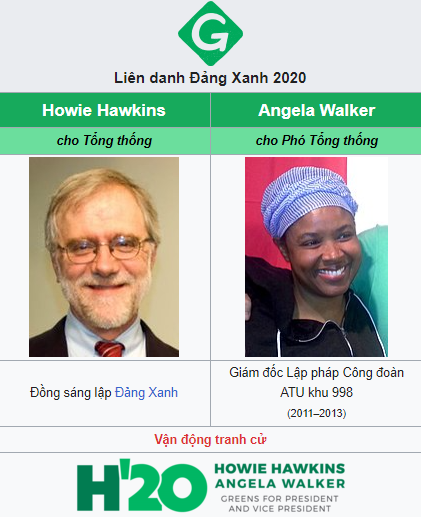
\includegraphics[width=0.6\textwidth]{Green_Candidates.png}
        \caption{Ứng cử viên Tổng thống và ứng cử viên Phó Tổng thống Đảng Xanh}
    \end{figure}

    \section{Trực quan hóa dữ liệu kết quả cuộc bầu cử Tổng thống năm 2020}

    Cuộc bầu cử tổng thống Mỹ năm 2020 là một cuộc bầu cử quốc gia để chọn tổng thống và Phó tổng thống Mỹ cho kỳ thứ 46. 
    Đảng Dân chủ và Đảng Cộng hòa đều có các ứng cử viên, với Joe Biden là ứng cử viên của Đảng Dân chủ và Donald Trump là ứng cử viên của Đảng Cộng hòa. 
    Cuộc bầu cử được tổ chức vào ngày 3 tháng 11 năm 2020 và kết quả chính thức được công bố vào ngày 7 tháng 11 năm 2020, Joe Biden đã đạt được sự thắng lợi với 306 phiếu Đại cử tri và Donald Trump đạt được 232 phiếu Đại cử tri.

    \begin{figure}[h!]
        \centering
        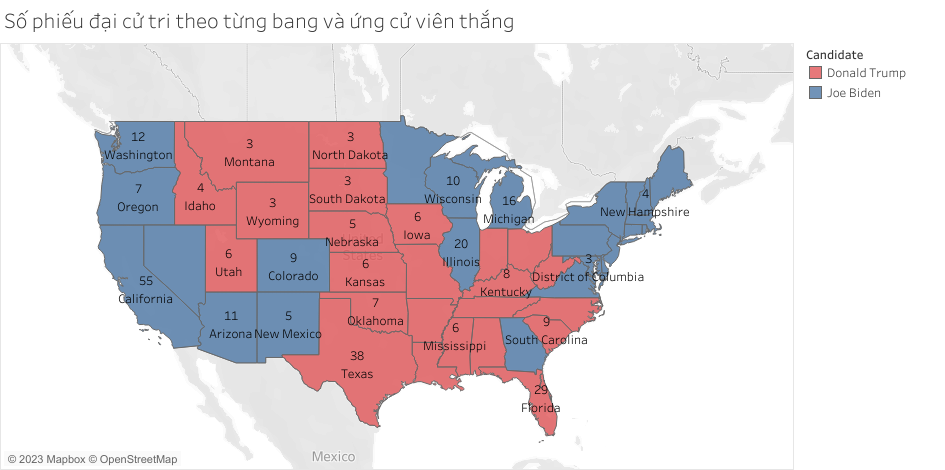
\includegraphics[width=0.9\textwidth]{Electoral_Votes_States.png}
        \caption{Số phiếu đại cử tri theo từng bang và ứng cử viên thắng}
    \end{figure}

    \begin{figure}[h!]
        \centering
        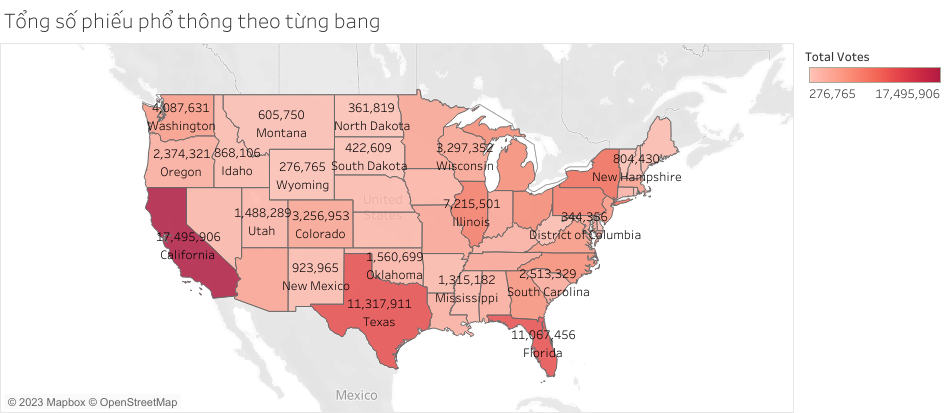
\includegraphics[width=0.9\textwidth]{Popular_Votes_States_by_Color.png}
        \caption{Tổng số phiếu phổ thông theo từng bang}
    \end{figure}

    \begin{figure}[h!]
        \centering
        \begin{subfigure}[b]{\textwidth}
            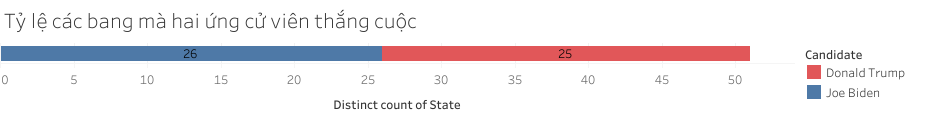
\includegraphics[width=0.9\textwidth]{figures/State_Candidate_Win.png}
            \caption{Số bang mà các ứng cử viên thắng}
        \end{subfigure}
        \vfill
        \begin{subfigure}[b]{\linewidth}
            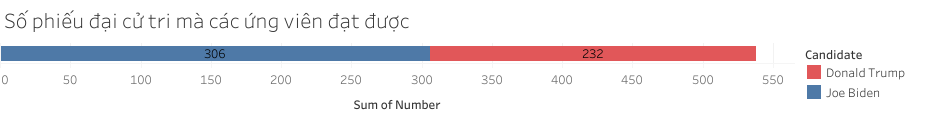
\includegraphics[width=0.9\linewidth]{figures/Electoral_Vote_Candidate_Win.png}
            \caption{Số phiếu Đại cử tri mà các ứng cử vien giành được}
        \end{subfigure}
        \caption{Kết quả chung cuộc của cuộc tranh cử Tổng thống Mỹ năm 2020}
    \end{figure}

    Trong cuộc bầu cử tổng thống Mỹ năm 2020, Joe Biden đã đạt được sự thắng lợi trong 26 bang, đạt được tổng cộng 306 phiếu Đại cử tri trong tổng số 538 phiếu Đại cử tri. 
    Donald Trump đã đạt được sự thắng lợi trong 25 bang, đạt được tổng cộng 232 phiếu Đại cử tri.

    Một số bang có một số lớn phiếu Đại cử tri và đại diện quan trọng trong cuộc bầu cử như Pennsylvania, Michigan và Wisconsin đã cho Joe Biden giành chiến thắng. 
    Còn một số bang có nhiều phiếu chốt như Texas, Florida và North Carolina mà ông Donald Trump giành chiến thắng.

    Tổng quan, cuộc bầu cử năm 2020 cho thấy sự chia rẽ trong cộng đồng Mỹ về những vấn đề như chính sách, sức khỏe và an ninh. 
    Kết quả cuộc bầu cử cho thấy rằng cộng đồng Mỹ đang phân tán về các vấn đề quan trọng.

    \begin{figure}[h!]
        \centering
        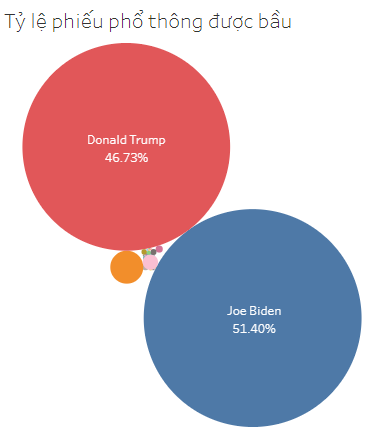
\includegraphics[width=0.6\textwidth]{Percentage_Total_Candidates_Bubble_Chart.png}
        \caption{Tỷ lệ phiếu phổ thông được bầu của từng ứng cử viên}
    \end{figure}

    Có một số bang mà các ứng viên đảng Cộng hòa gần như không có cơ hội thắng, chẳng hạn như California, New York, và Washington. 
    Tuy nhiên, tình hình cục bộ tại mỗi bang có thể khác nhau, và các yếu tố như tình trạng kinh tế, chính sách, và phong trào của các đảng cũng có thể ảnh hưởng đến kết quả bầu cử tại các bang này.

    \begin{figure}[h!]
        \centering
        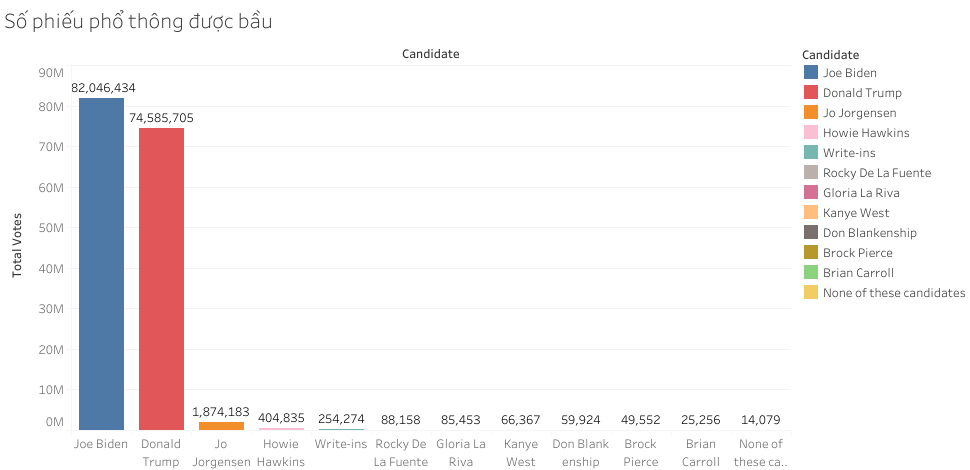
\includegraphics[width=0.9\textwidth]{Total_Popular_Votes_Candidates_Bar_Chart.png}
        \caption{Tổng số phiếu phổ thông được bầu của từng ứng cử viên}
    \end{figure}

    \begin{figure}[h!]
        \centering
        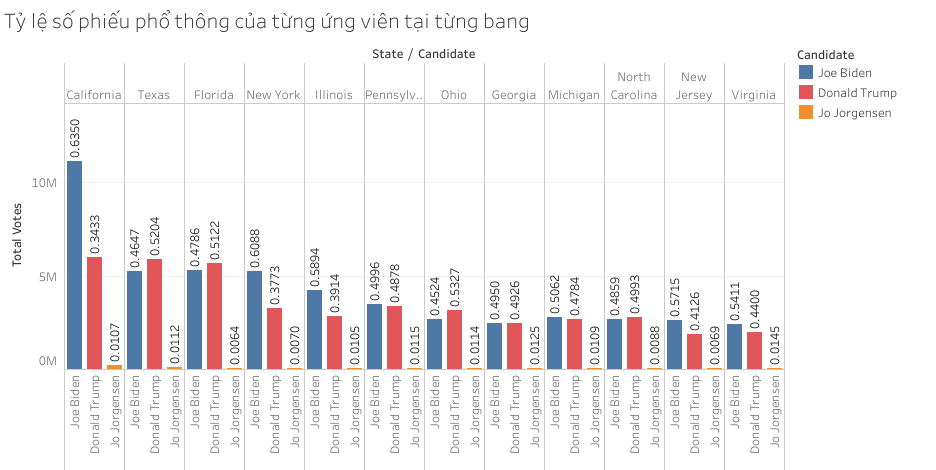
\includegraphics[width=0.9\textwidth]{Percentage_Popular_Votes_Candidates_by_States.png}
        \caption{Tỷ lệ số phiếu phổ thông của từng ứng viên tại từng bang}
    \end{figure}

    Cuộc bầu cử Tổng thống Hoa Kỳ năm 2020 là một cuộc đua có tính cạnh tranh cao, với cựu Phó Tổng thống Joe Biden giành được 306 phiếu Đại cử tri so với 232 của Tổng thống đương nhiệm Donald Trump. 
    Biden cũng giành được số phiếu phổ thông với tổng cộng 81.283.485 phiếu bầu (51,3\%) so với 74.223.975 phiếu bầu của Trump (46,8\%).

    Về phân bổ số phiếu phổ thông theo bang, Biden giành được đa số phiếu phổ thông ở 25 bang và Quận Columbia, trong khi Trump giành được đa số phiếu phổ thông ở 25 bang. 
    Một số bang quan trọng mà Biden giành chiến thắng California, New York và Pennsylvania, trong khi Trump thể hiện tốt ở Texas, Florida và Ohio.

    Điều quan trọng cần lưu ý là phổ thông đầu phiếu chỉ là một khía cạnh của cuộc bầu cử và người chiến thắng trong cuộc bầu cử được quyết định bởi Đại cử tri đoàn, phân bổ phiếu bầu cho mỗi bang dựa trên đại diện của bang đó trong Quốc hội. 
    Điều này có nghĩa là việc phân phối phiếu Đại cử tri theo bang có thể rất khác so với việc phân phối phiếu phổ thông.

    \begin{figure}[h!]
        \centering
        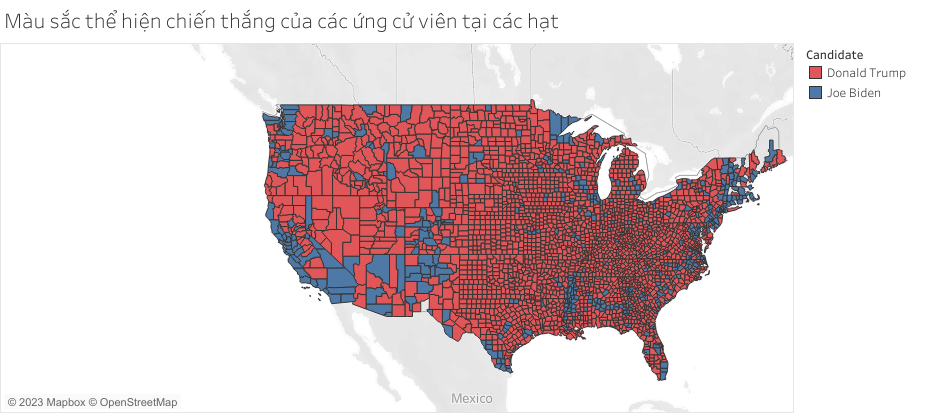
\includegraphics[width=0.9\textwidth]{County_Candidate_Win.png}
        \caption{Màu sắc thể hiện chiến thắng của các ứng cử viên tại các hạt}
    \end{figure}

    \begin{figure}[h!]
        \centering
        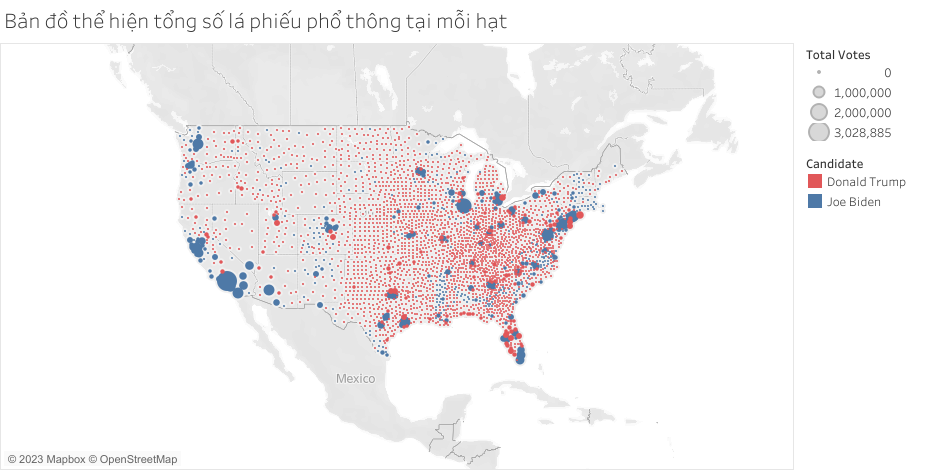
\includegraphics[width=0.9\textwidth]{County_Total_Vote_Circle.png}
        \caption{Bản đồ thể hiện tổng số lá phiếu phổ thông tại mỗi hạt}
    \end{figure}

    Tại Hoa Kỳ, Tổng thống được bầu không dựa trên số hạt giành được, mà dựa trên số phiếu đại cử tri giành được. 
    Mỗi bang được phân bổ một số phiếu Đại cử tri nhất định dựa trên dân số của bang đó và ứng cử viên nào giành được đa số phiếu bầu ở bang này sẽ giành được tất cả phiếu đại cử tri của bang đó.
    Ông Joe Biden đã giành được tổng cộng 306 phiếu đại cử tri so với 232 phiếu đại cử tri của Donald Trump, mặc dù Trump đã giành được đa số hạt ở một số bang. 
    Điều này cho thấy rằng Biden đã giành được các bang quan trọng có dân số cao, giúp ông có nhiều phiếu đại cử tri hơn và cuối cùng dẫn đến chiến thắng của ông trong cuộc bầu cử.

    \begin{figure}[h!]
        \centering
        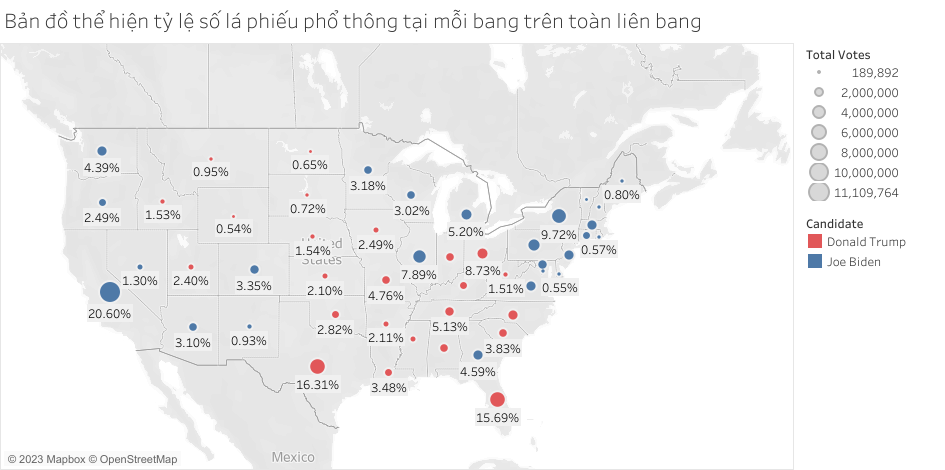
\includegraphics[width=0.9\textwidth]{State_Percentage_Vote_Circle.png}
        \caption{Bản đồ thể hiện tỷ lệ số lá phiếu phổ thông tại mỗi bang trên toàn liên bang}
    \end{figure}

    \begin{figure}[h!]
        \centering
        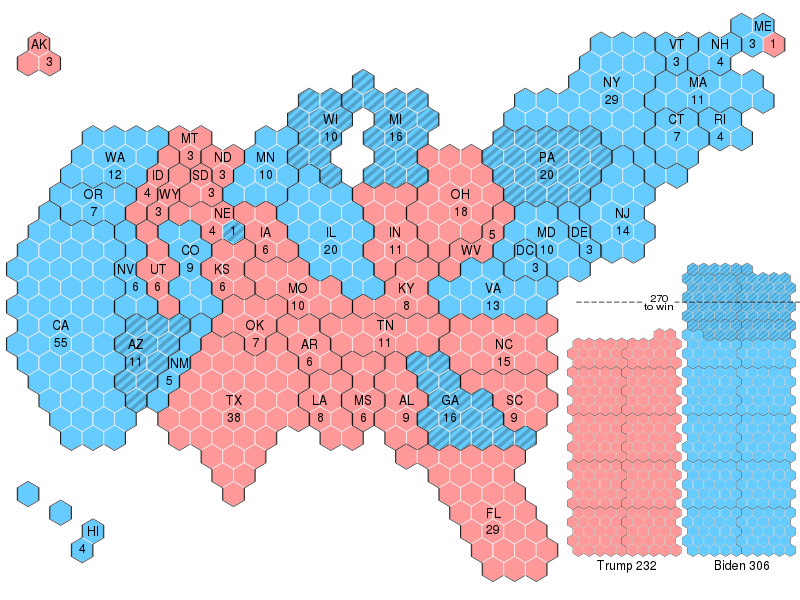
\includegraphics[width=0.9\textwidth]{State_Total_Vote_Cartogram.png}
        \caption{Cartogram thể hiện tổng số lá phiếu phổ thông tương ứng với các ứng cử viên thắng cuộc}
    \end{figure}

    \begin{figure}[h!]
        \centering
        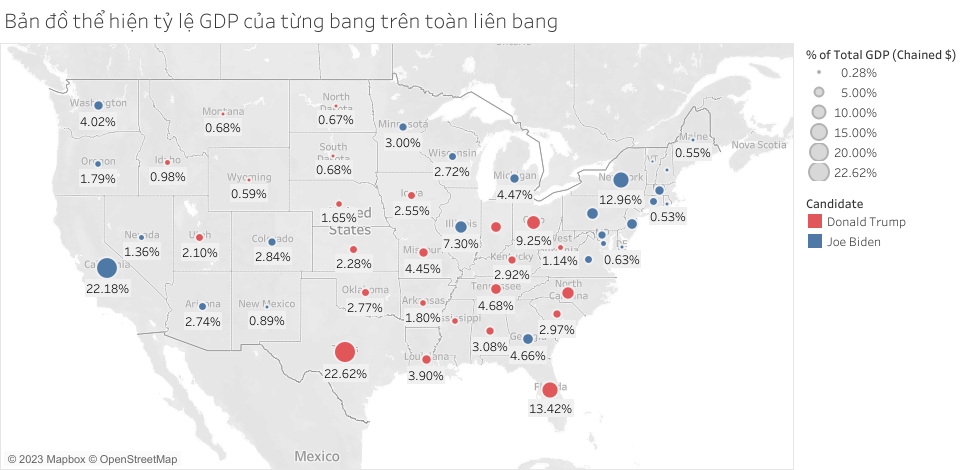
\includegraphics[width=0.9\textwidth]{figures/State_Percentage_GDP_Circle.png}
        \caption{Tỷ lệ GDP của tiểu bang trên toàn liên bang}
    \end{figure}

    \begin{figure}[h!]
        \centering
        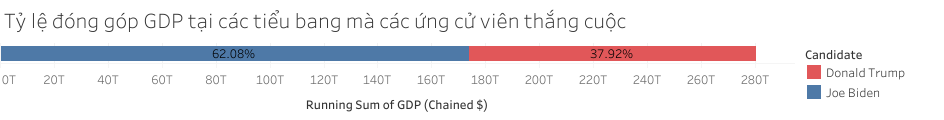
\includegraphics[width=0.9\textwidth]{State_Percentage_GDP_Candidate.png}
        \caption{Tỷ lệ đóng góp GDP tại các tiểu bang mà các ứng cử viên thắng}
    \end{figure}

    \begin{figure}[h!]
        \centering
        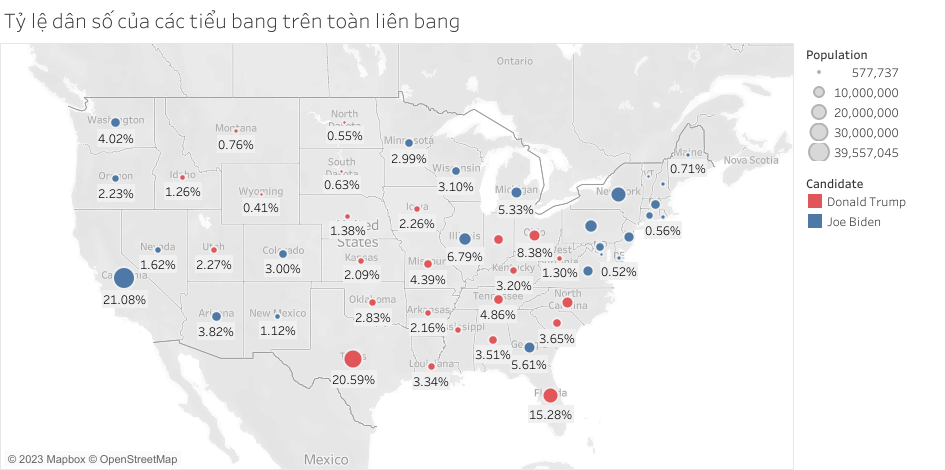
\includegraphics[width=0.9\textwidth]{State_Percentage_Population_Circle.png}
        \caption{Tỷ lệ dân số của tiểu bang trên toàn liên bang}
    \end{figure}

    \begin{figure}[h!]
        \centering
        \includegraphics[width=0.9\textwidth]{figures/State_Percentage_Population_Candidate.png}
        \caption{Tỷ lệ đóng góp dân số tại các tiểu bang mà các ứng cử viên thắng}
    \end{figure}

    \begin{figure}[h!]
        \centering
        \includegraphics[width=0.9\textwidth]{figures/County_Total_Percentage_Candidate_Win.png}
        \caption{Tỷ lệ thắng trên các hạt của từng ứng cử viên}
    \end{figure}

    \begin{figure}[h!]
        \centering
        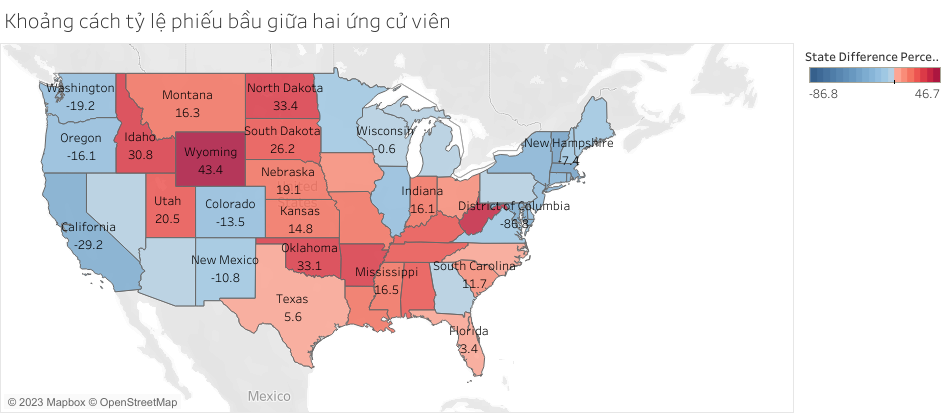
\includegraphics[width=0.9\textwidth]{figures/State_Difference_Percentage_Total_Vote_Two_Candidate.png}
        \caption{Khoảng cách tỷ lệ phiếu bầu giữa hai ứng cử viên tại các bang}
    \end{figure}

    \begin{figure}[h!]
        \centering
        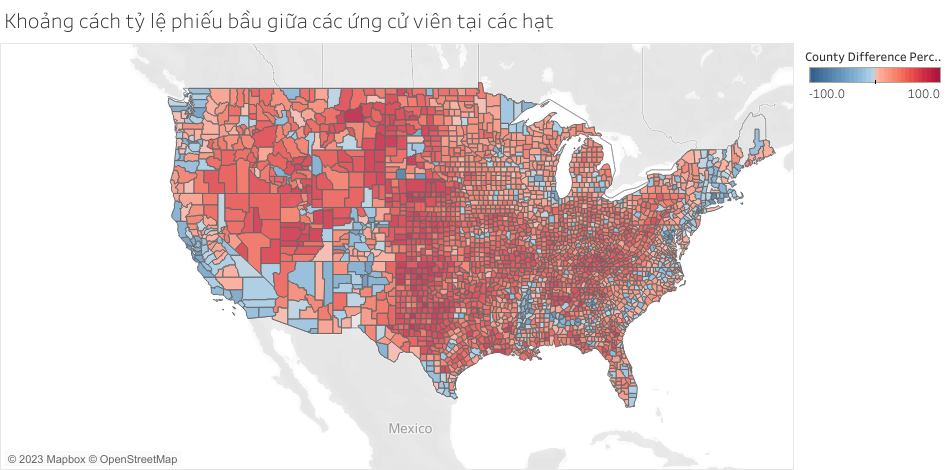
\includegraphics[width=0.9\textwidth]{figures/County_Difference_Percentage_Total_Vote_Two_Candidate.png}
        \caption{Khoảng cách tỷ lệ phiếu bầu giữa các ứng cử viên tại các hạt}
    \end{figure}

    \begin{figure}[h!]
        \centering
        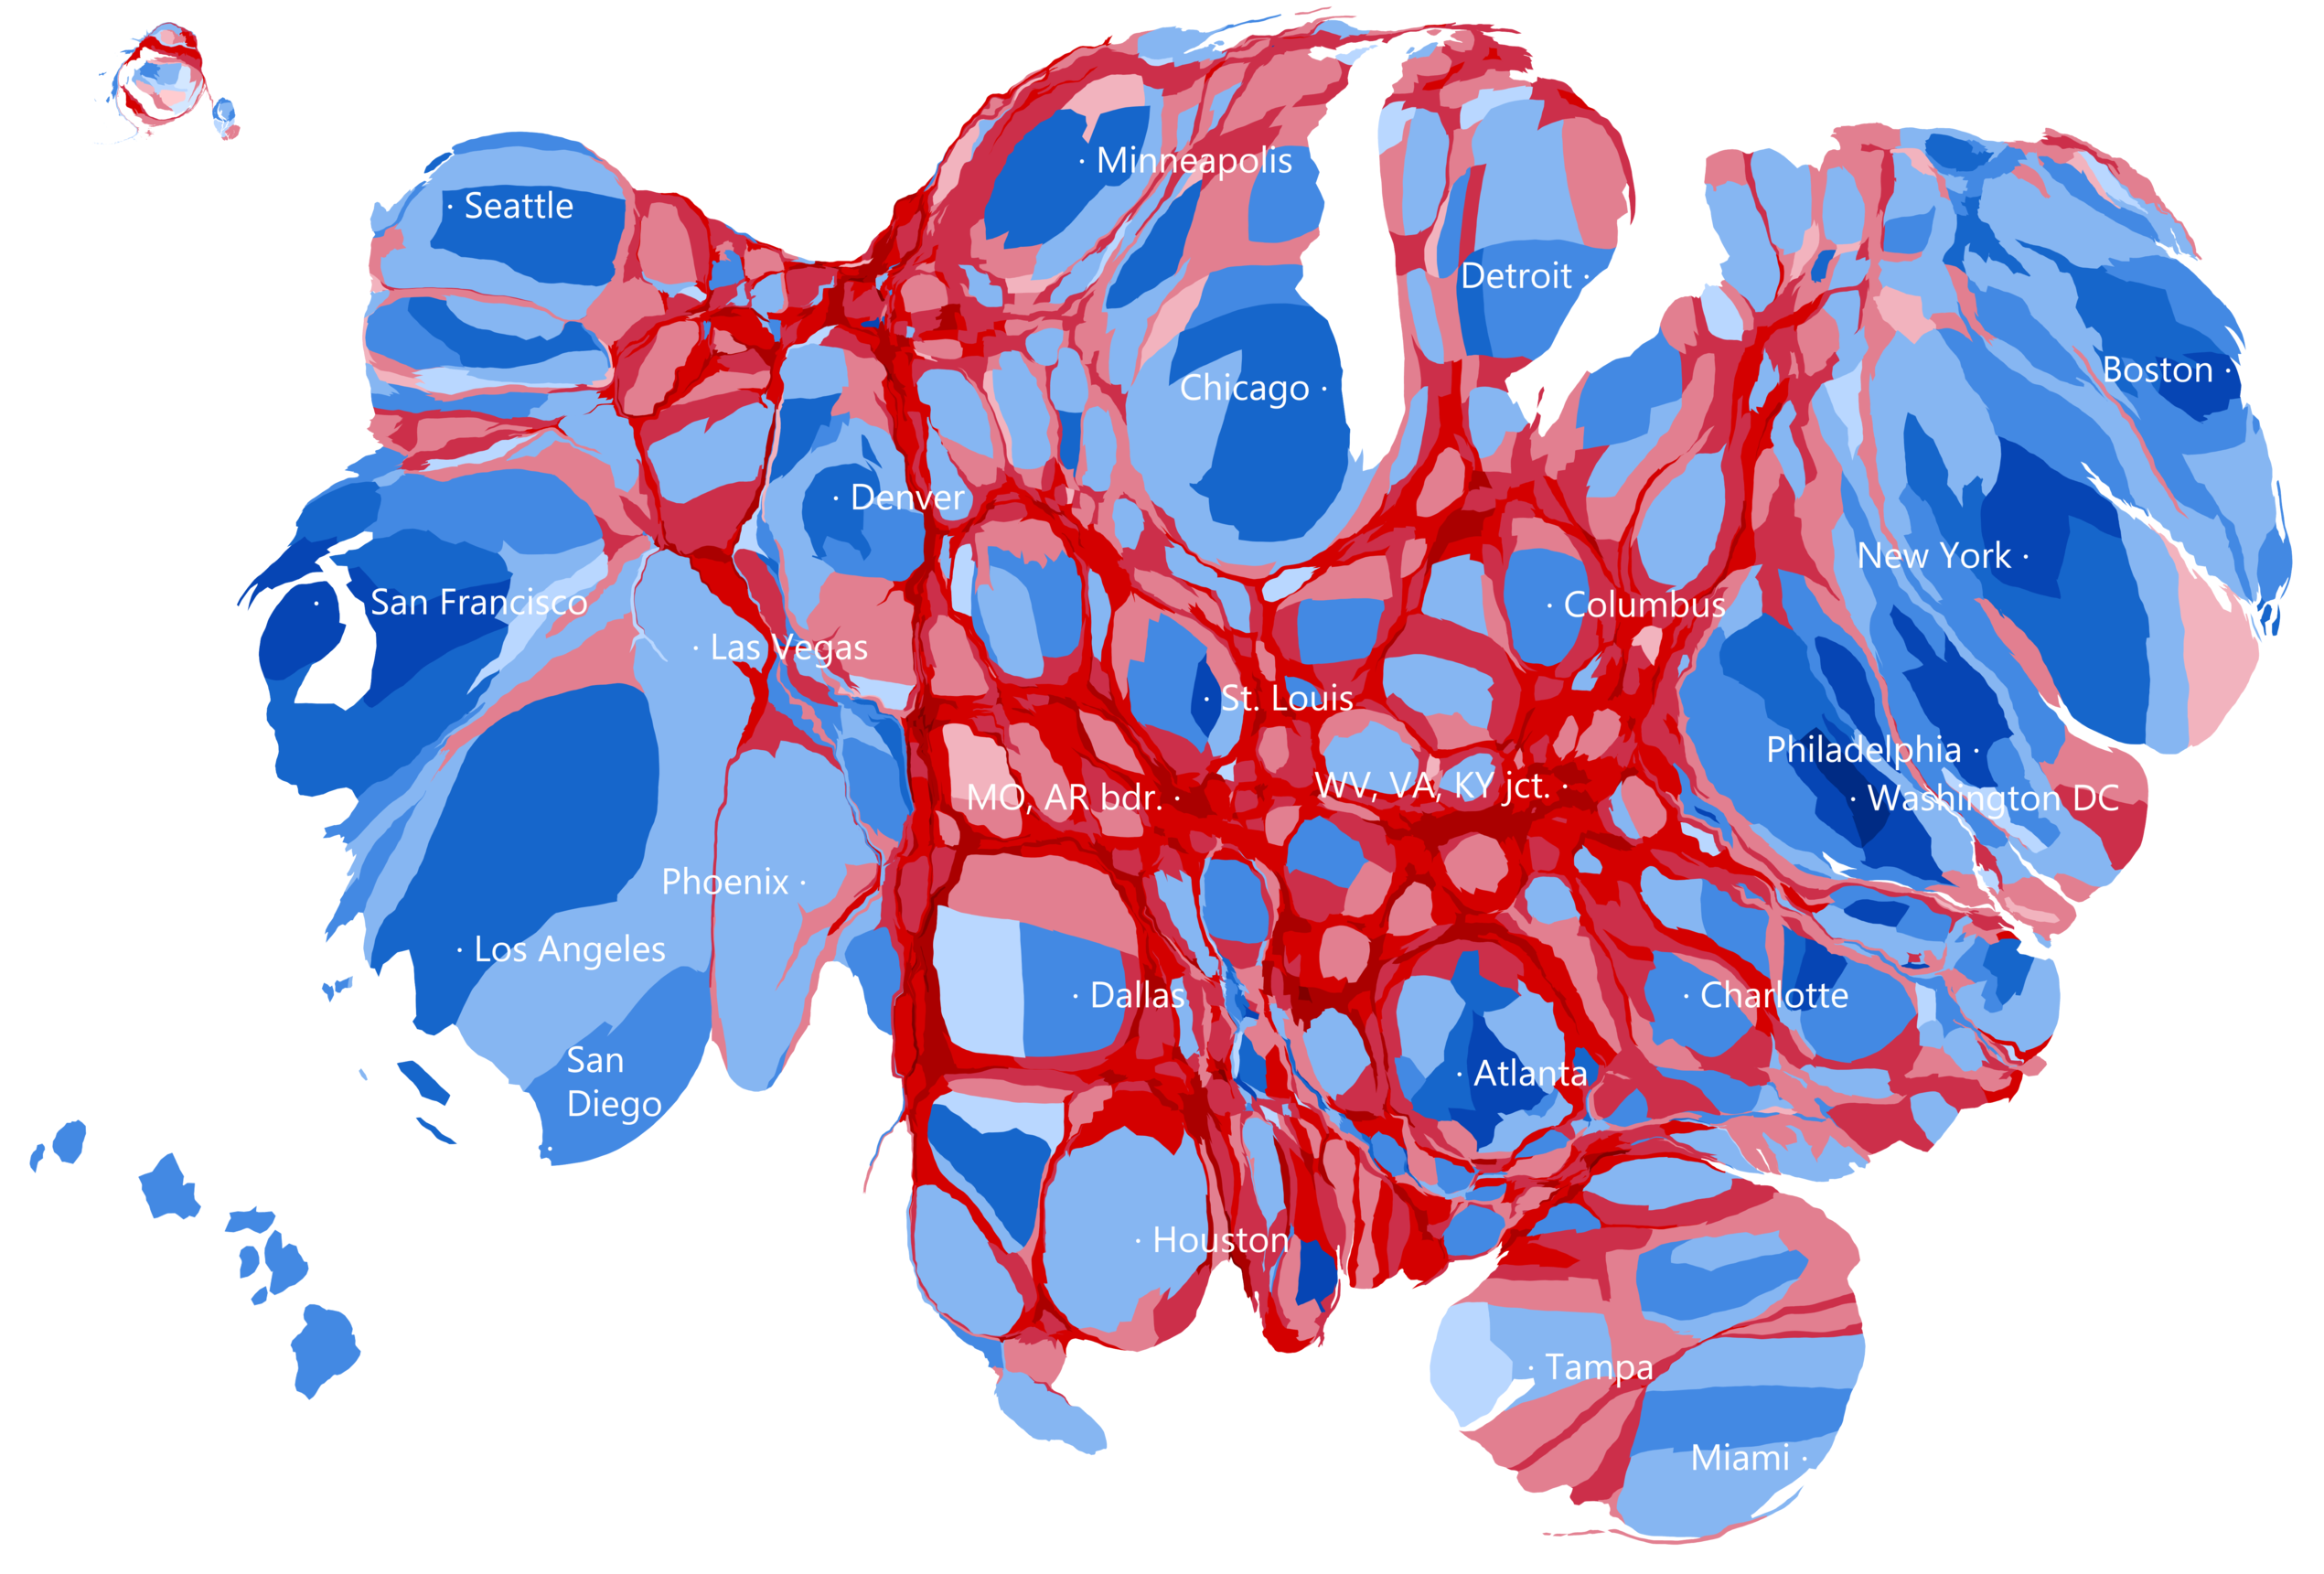
\includegraphics[width=0.9\textwidth]{figures/County_Total_Vote_Cartogram.png}
        \caption{Cartogram thể hiện tổng số lá phiếu phổ thông tương ứng với các ứng cử viên thắng cuộc trên cấp độ hạt}
    \end{figure}

    Trong Cuộc bầu cử Tổng thống Hoa Kỳ năm 2020, ứng cử viên Đảng Cộng hòa, Donald Trump, đã giành chiến thắng ở đa số hạt, với chiến thắng ở hơn 3000 hạt trên khắp Hoa Kỳ. 
    Tuy nhiên, điều này không chuyển thành đa số phiếu phổ thông, vì ứng cử viên Đảng Dân chủ, Joe Biden, đã giành chiến thắng với 306 phiếu đại cử tri so với 232 của Trump. 
    Sự phân bổ số phiếu phổ thông, kết hợp với cách thức hoạt động của Đại cử tri đoàn, có nghĩa là Biden đã thắng cuộc bầu cử mặc dù thua đa số các hạt.

    \begin{figure}[h!]
        \centering
        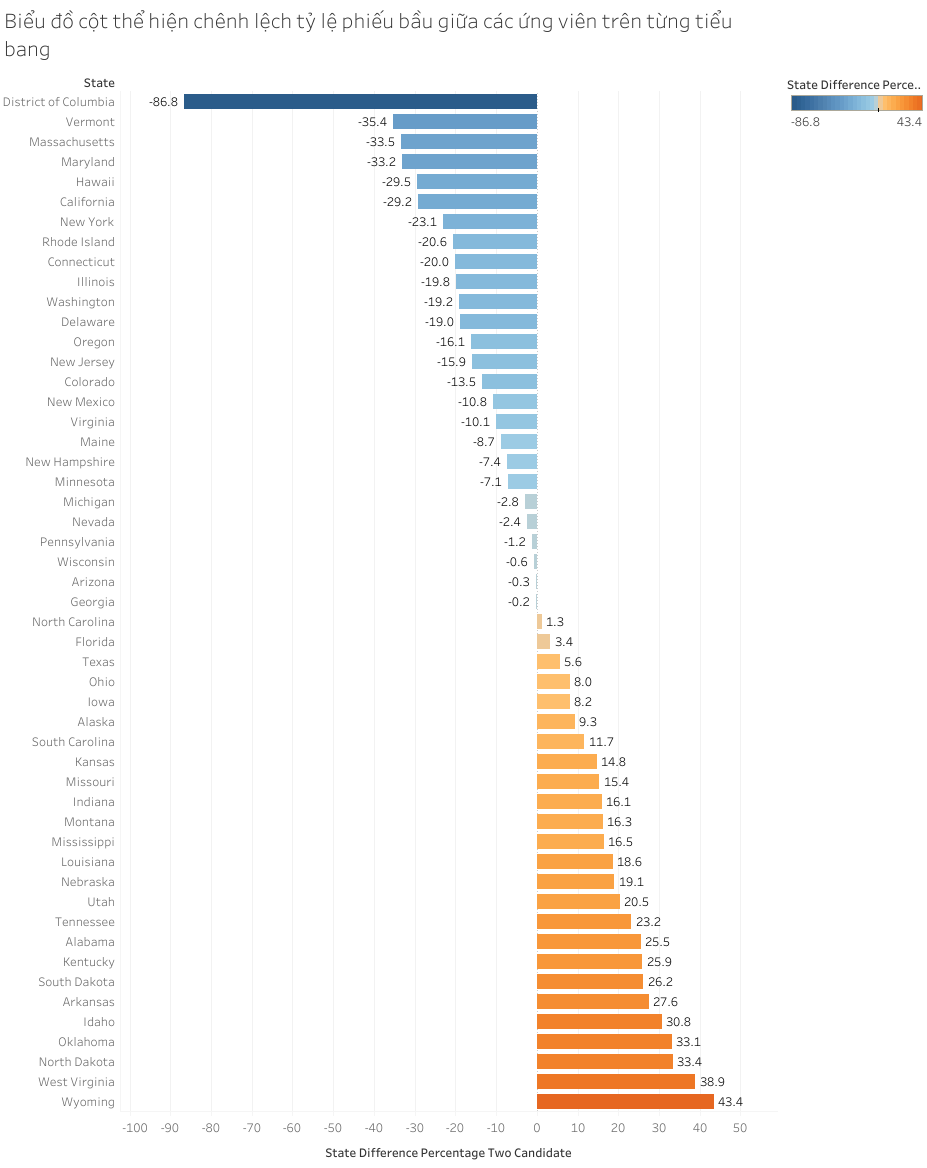
\includegraphics[width=0.9\textwidth]{figures/State_Difference_Percentage_Total_Vote_Two_Candidate_Bar_Chart.png}
        \caption{Biểu đồ cột thể hiện chênh lệch tỷ lệ phiếu bầu giữa các ứng viên trên từng tiểu bang}
    \end{figure}

    Một số bang được coi là "chiến địa" do chúng có sức mạnh tác động lớn đến kết quả cuộc bầu cử. 
    Một số trong những bang này bao gồm:

    \begin{itemize}
        \item Pennsylvania
        \item Michigan
        \item Wisconsin
        \item Arizona
        \item Georgia
    \end{itemize}

    Một số bang chỉ có tỷ lệ phân biệt rất nhỏ giữa hai ứng cử viên.
    Tất cả các bang trên đều là bang mà Joe Biden đã đạt được sự thắng lợi.

    Cuộc bầu cử tại các bang chiến địa đã trở thành một trong những chủ đề chính trong cuộc bầu cử, với cả hai bên cố gắng đầu tư nhiều thời gian và công sức để giành sự thắng lợi trong những bang này. 
    Các nhà chính trị đều nhìn thấy giá trị quan trọng của việc giành được sự thắng lợi trong những bang chiến địa này, vì nó có thể quyết định chiến thắng trong cuộc bầu cử.

    \begin{figure}[h!]
        \centering
        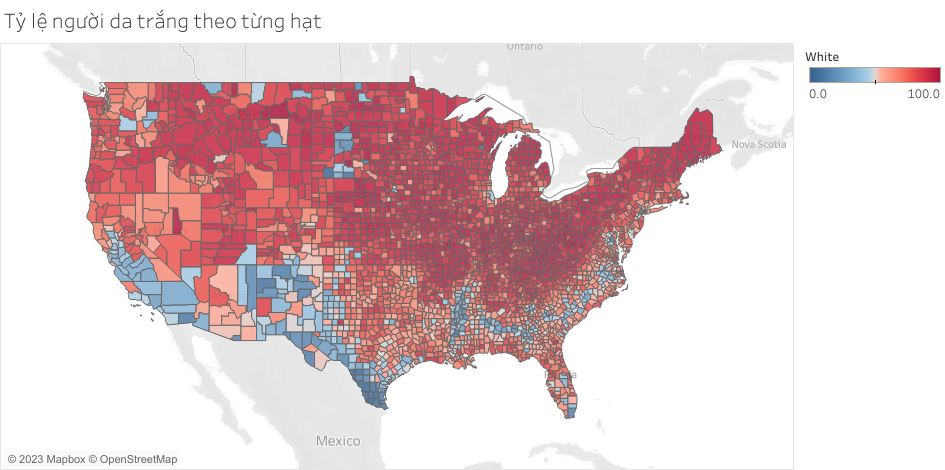
\includegraphics[width=0.9\textwidth]{figures/County_Percentage_White_People.png}
        \caption{Tỷ lệ người da trắng theo từng hạt}
    \end{figure}

    \begin{figure}[h!]
        \centering
        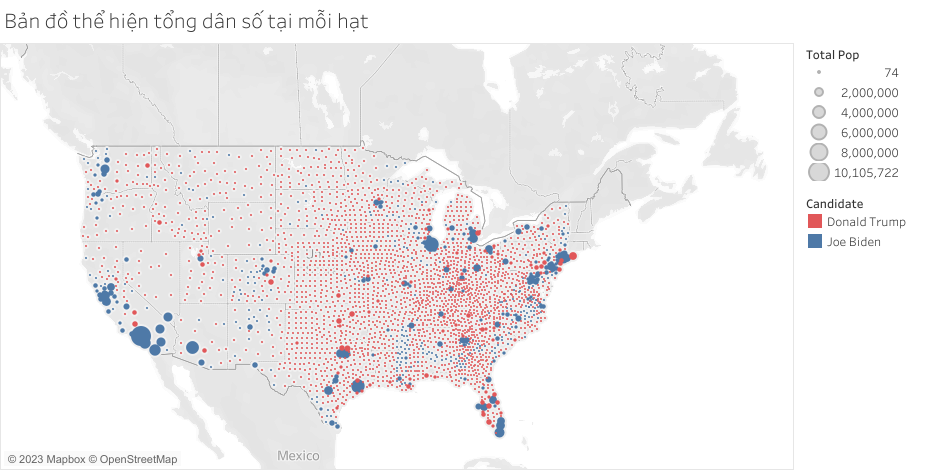
\includegraphics[width=0.9\textwidth]{figures/County_Total_Population_Circle.png}
        \caption{Bản đồ thể hiện tổng dân số tại mỗi hạt}
    \end{figure}

    \begin{figure}[h!]
        \centering
        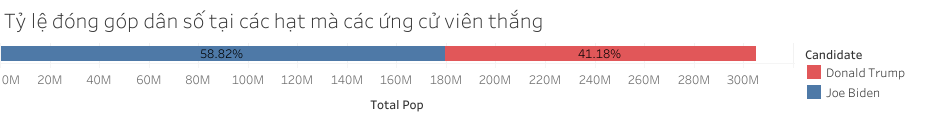
\includegraphics[width=0.9\textwidth]{figures/County_Percentage_Population_Candidate.png}
        \caption{Tỷ lệ đóng góp dân số tại các hạt mà các ứng cử viên thắng}
    \end{figure}

    \begin{figure}[h!]
        \centering
        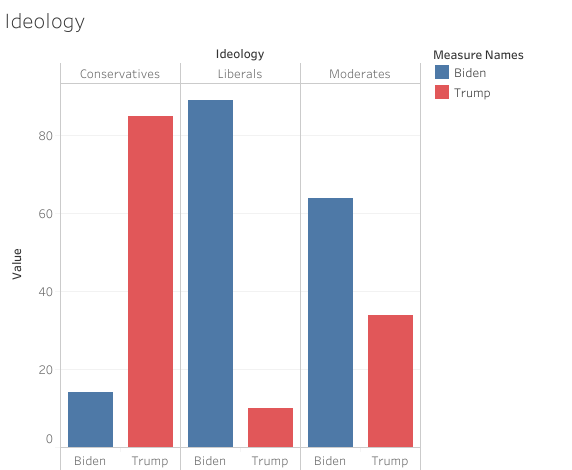
\includegraphics[width=0.6\textwidth]{figures/Ideology.png}
        \caption{Tỷ lệ ủng hộ ứng cử viên theo quan điểm chính trị}
    \end{figure}

    \begin{figure}[h!]
        \centering
        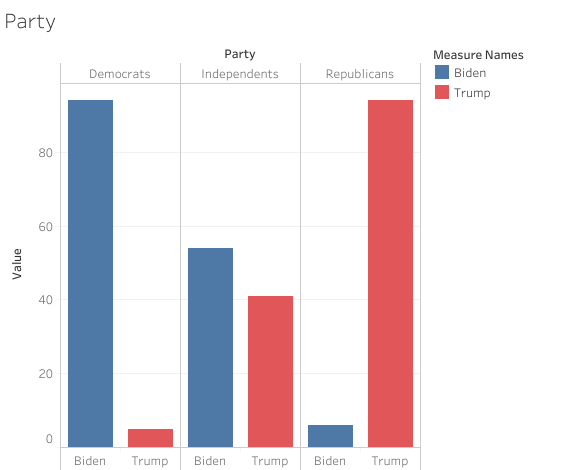
\includegraphics[width=0.6\textwidth]{figures/Party.png}
        \caption{Tỷ lệ ủng hộ ứng cử viên theo đảng phái chính trị}
    \end{figure}

    \begin{figure}[h!]
        \centering
        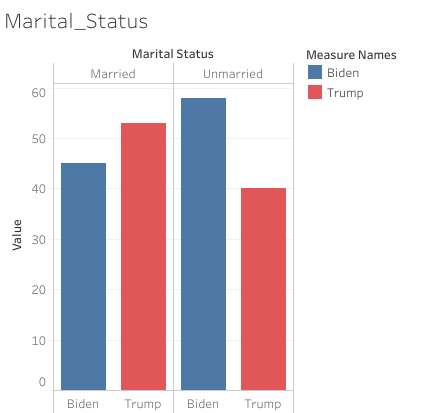
\includegraphics[width=0.6\textwidth]{figures/Marital_Status.png}
        \caption{Tỷ lệ ủng hộ ứng cử viên theo tình trạng hôn nhân}
    \end{figure}

    \begin{figure}[h!]
        \centering
        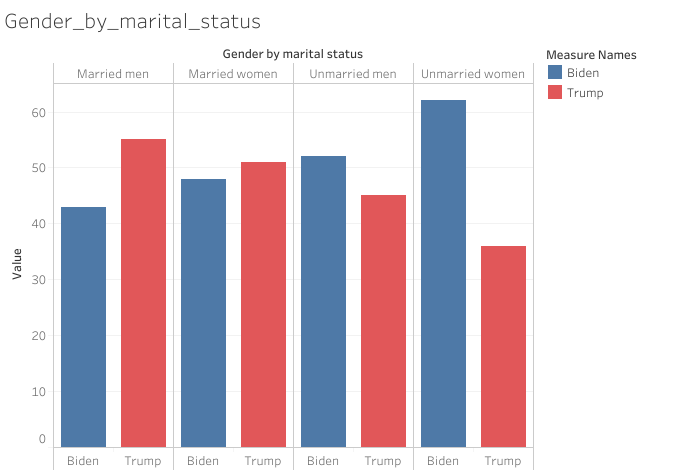
\includegraphics[width=0.6\textwidth]{figures/Gender_by_marital_status.png}
        \caption{Tỷ lệ ủng hộ ứng cử viên theo giới tính và tình trạng hôn nhân}
    \end{figure}

    \begin{figure}[h!]
        \centering
        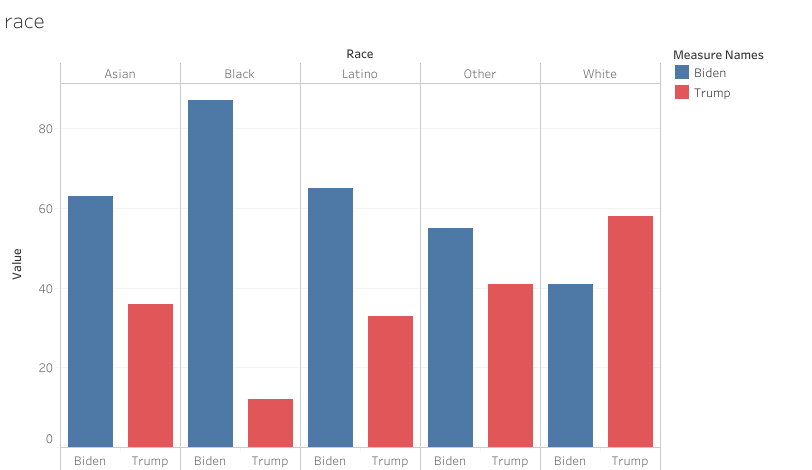
\includegraphics[width=0.6\textwidth]{figures/race.png}
        \caption{Tỷ lệ ủng hộ ứng cử viên theo chủng tộc}
    \end{figure}

    \begin{figure}[h!]
        \centering
        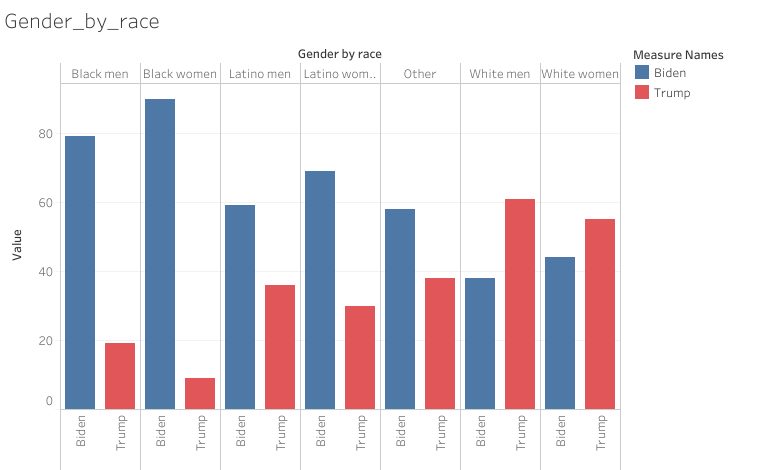
\includegraphics[width=0.6\textwidth]{figures/Gender_by_race.png}
        \caption{Tỷ lệ ủng hộ ứng cử viên theo giới tính và chủng tộc}
    \end{figure}

    \begin{figure}[h!]
        \centering
        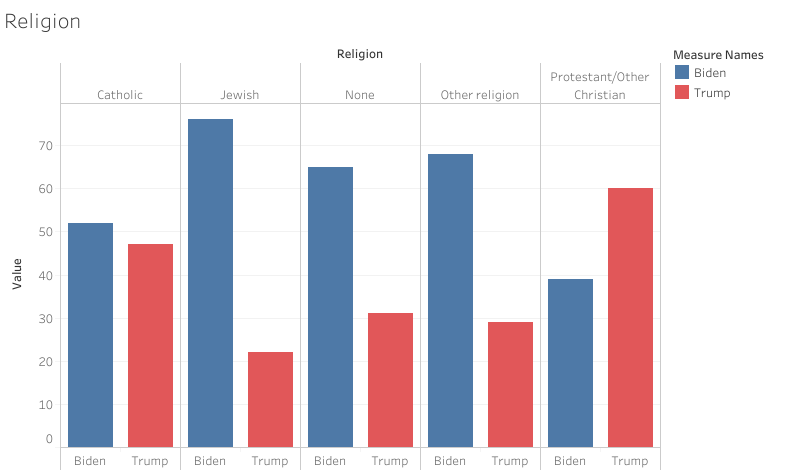
\includegraphics[width=0.6\textwidth]{figures/Religion.png}
        \caption{Tỷ lệ ủng hộ ứng cử viên theo tôn giáo}
    \end{figure}

    \begin{figure}[h!]
        \centering
        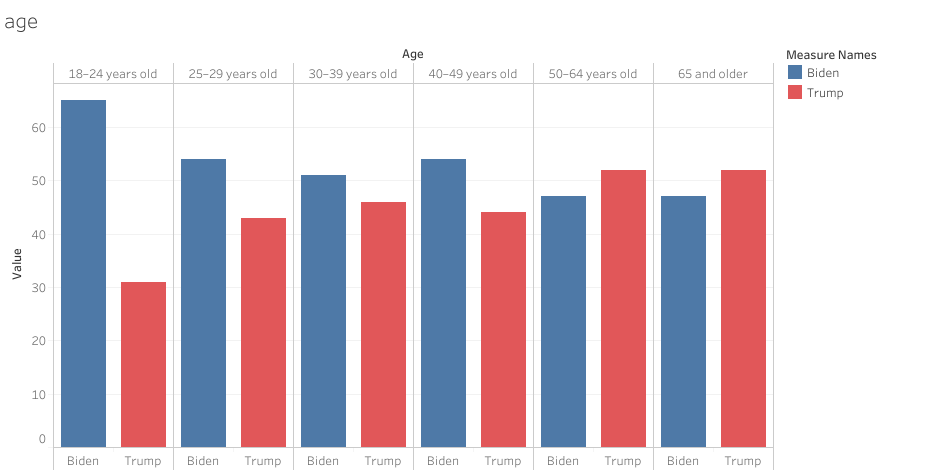
\includegraphics[width=0.6\textwidth]{figures/age.png}
        \caption{Tỷ lệ ủng hộ ứng cử viên theo độ tuổi}
    \end{figure}

    \begin{figure}[h!]
        \centering
        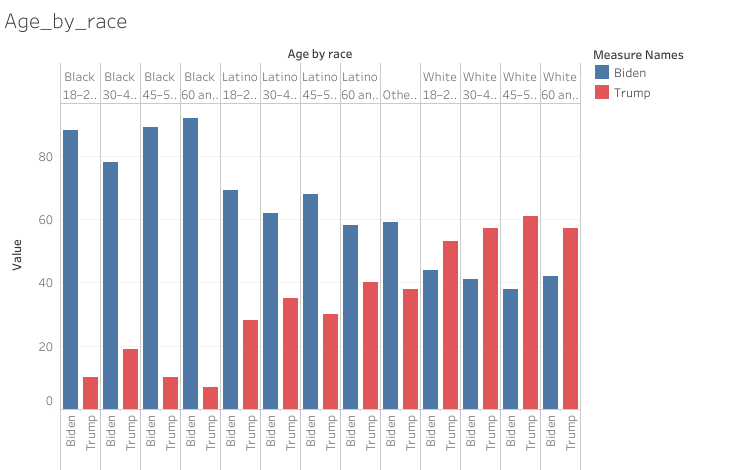
\includegraphics[width=0.6\textwidth]{figures/Age_by_race.png}
        \caption{Tỷ lệ ủng hộ ứng cử viên theo độ tuổi và chủng tộc}
    \end{figure}

    Tỷ lệ ủng hộ của hai ứng cử viên Joe Biden và Donald Trump có sự chênh lệch về mặt dân số.

    Joe Biden đã đạt được sự ủng hộ từ những nhóm dân số như người trẻ, người Mỹ gốc Latinh và người Mỹ gốc da màu. 
    Donald Trump đã đạt được sự ủng hộ từ những nhóm dân số như người lớn tuổi, người Mỹ gốc châu Âu và người Mỹ gốc da trắng.

    Tuy nhiên, cả hai ứng cử viên đều đã cố gắng giành được sự ủng hộ của mọi nhóm dân số, từ những nhóm dân số lớn đến những nhóm nhỏ hơn. 
    Cuộc bầu cử đã chứng minh rằng cả hai ứng cử viên đều có sức mạnh và năng lực tại những nơi khác nhau trên đất nước.

    \begin{figure}[h!]
        \centering
        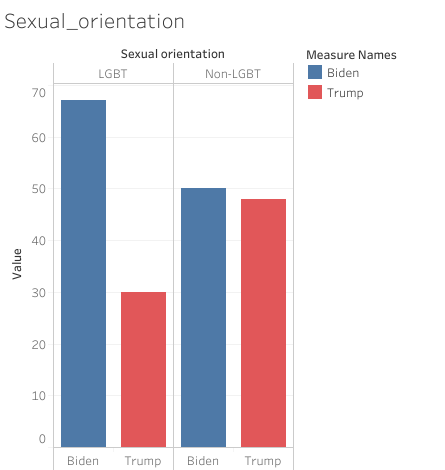
\includegraphics[width=0.6\textwidth]{figures/Sexual_orientation.png}
        \caption{Tỷ lệ ủng hộ ứng cử viên theo xu hướng giới tính}
    \end{figure}

    \begin{figure}[h!]
        \centering
        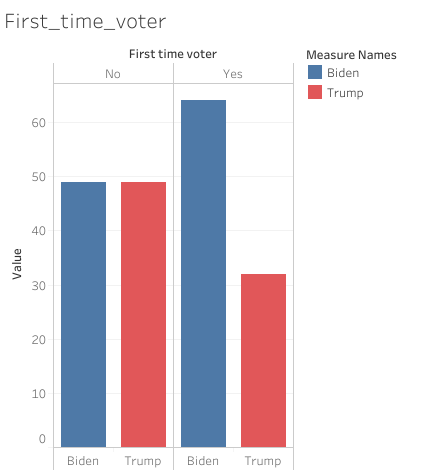
\includegraphics[width=0.6\textwidth]{figures/First_time_voter.png}
        \caption{Tỷ lệ ủng hộ ứng cử viên theo số lần đi bỏ phiếu}
    \end{figure}

    \begin{figure}[h!]
        \centering
        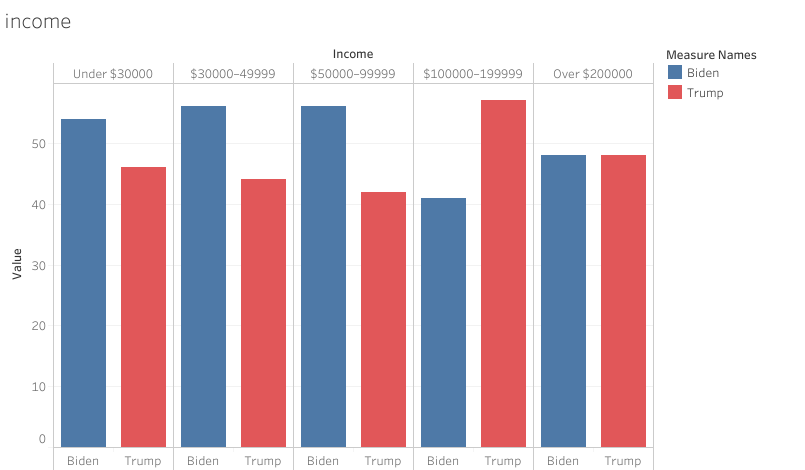
\includegraphics[width=0.6\textwidth]{figures/income.png}
        \caption{Tỷ lệ ủng hộ ứng cử viên theo thu nhập}
    \end{figure}

    \begin{figure}[h!]
        \centering
        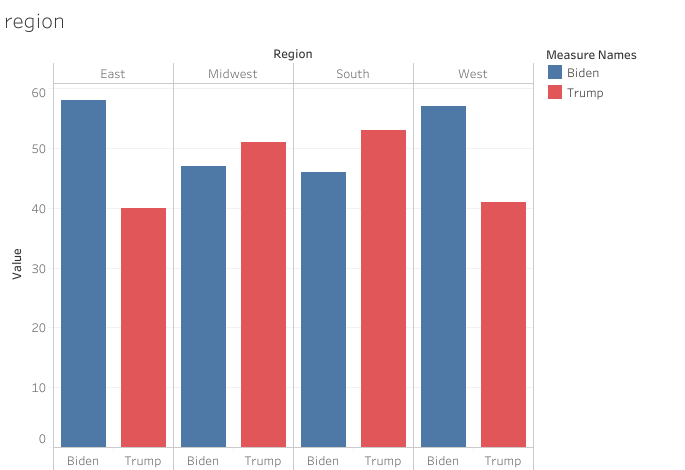
\includegraphics[width=0.6\textwidth]{figures/region.png}
        \caption{Tỷ lệ ủng hộ ứng cử viên theo khu vực}
    \end{figure}

    \begin{figure}[h!]
        \centering
        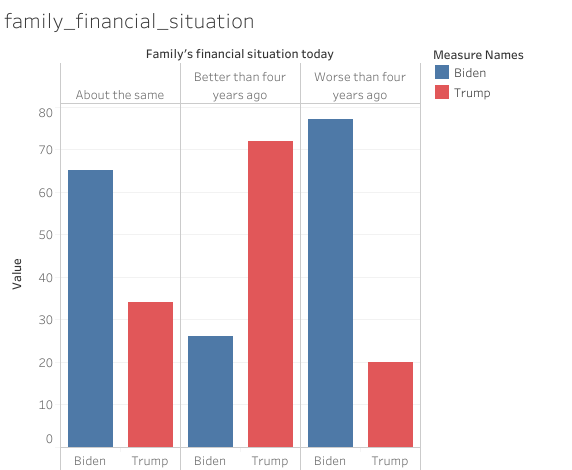
\includegraphics[width=0.6\textwidth]{figures/family_financial_situation.png}
        \caption{Tỷ lệ ủng hộ ứng cử viên theo tình trạng tài chính}
    \end{figure}

    \begin{figure}[h!]
        \centering
        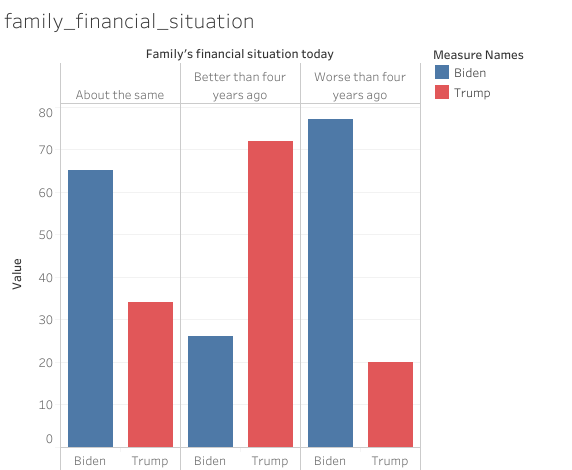
\includegraphics[width=0.6\textwidth]{figures/family_financial_situation.png}
        \caption{Tỷ lệ ủng hộ ứng cử viên theo phục vụ quân ngũ}
    \end{figure}

    \begin{figure}[h!]
        \centering
        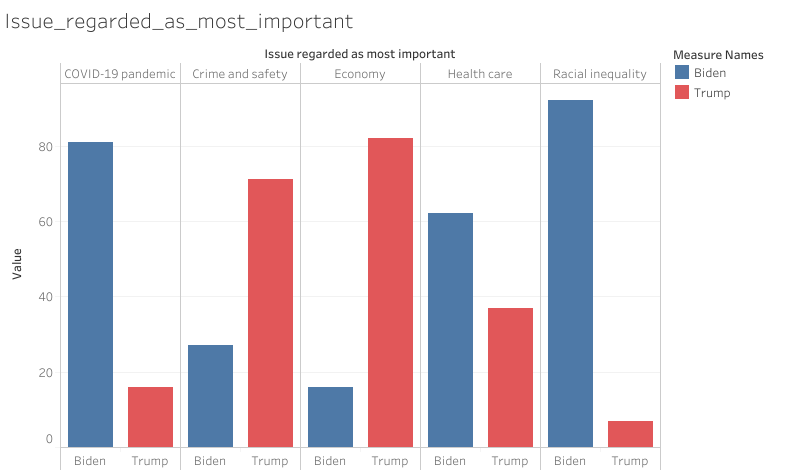
\includegraphics[width=0.6\textwidth]{figures/Issue_regarded_as_most_important.png}
        \caption{Tỷ lệ ủng hộ ứng cử viên theo cách nhìn nhận các vấn đề xã hội}
    \end{figure}


    Đại dịch COVID-19 đã có một sức ảnh hưởng lớn đến kết quả cuộc bầu cử Tổng thống Mỹ năm 2020. 
    Một trong những yếu tố quan trọng là việc chính phủ đã cố gắng để giải quyết vấn đề về sức khỏe và kinh tế mà đại dịch đã gây ra.
    Cuộc bầu cử đã trở thành một phần của các cuộc tranh luận về cách để giải quyết đại dịch và cách để hỗ trợ những người bị ảnh hưởng. 
    Cả hai ứng cử viên đều đã cố gắng để trình bày các giải pháp của mình cho các vấn đề này và giành được sự ủng hộ của cộng đồng.
    Ngoài ra, đại dịch COVID-19 cũng đã ảnh hưởng đến cách mà cuộc bầu cử được thực hiện, bao gồm việc giới hạn số lượng người cho phép tại các điểm bầu cử và việc tăng trưởng số lượng người bầu cử qua bầu cử trực tuyến.

    Nền kinh tế là một vấn đề chính trong Cuộc bầu cử Tổng thống Hoa Kỳ năm 2020. 
    Cả hai ứng cử viên Joe Biden và Donald Trump đều có những kế hoạch và đề xuất khác nhau để giải quyết các mối quan ngại về kinh tế. 
    Biden tập trung vào nhu cầu đầu tư của chính phủ để thúc đẩy tăng trưởng kinh tế, bao gồm đầu tư vào cơ sở hạ tầng, năng lượng sạch và chăm sóc sức khỏe. 
    Ông cũng đề xuất các biện pháp hỗ trợ các doanh nghiệp nhỏ, tăng khả năng tiếp cận với dịch vụ chăm sóc sức khỏe hợp túi tiền và tăng mức lương tối thiểu. 
    Mặt khác, Trump đã vận động tranh cử dựa trên thành tích tăng trưởng kinh tế mạnh mẽ và tạo việc làm trước đại dịch COVID-19, đồng thời hứa sẽ tiếp tục thực hiện các chính sách hỗ trợ doanh nghiệp và giảm bớt các quy định mà ông cho là cản trở tăng trưởng kinh tế. 
    Nền kinh tế bị ảnh hưởng nặng nề bởi đại dịch COVID-19, điều này làm gia tăng cuộc tranh luận về phản ứng thích hợp từ chính phủ liên bang.

    Về vấn đề môi trường, ông Joe Biden đã đề xuất một kế hoạch toàn diện để chống biến đổi khí hậu, bao gồm đầu tư vào năng lượng tái tạo, tăng các quy định về khí thải và tái gia nhập Hiệp định Paris. 
    Ông cũng hứa sẽ ưu tiên vấn đề môi trường, đảm bảo rằng các cộng đồng da màu và cộng đồng có thu nhập thấp không bị ảnh hưởng nặng nề bởi các hiểm họa môi trường.
    Mặt khác, ông Donald Trump đã hủy bỏ một số quy định về môi trường, bao gồm cả những quy định liên quan đến ô nhiễm không khí và nước, như một phần nỗ lực của chính quyền ông nhằm thúc đẩy nền kinh tế và giảm sự can thiệp của chính phủ vào hoạt động kinh doanh. 
    Trump ủng hộ việc tăng cường sản xuất năng lượng trong nước, bao gồm khoan dầu khí, đồng thời thực hiện các bước để giảm quyền hạn của Cơ quan Bảo vệ Môi trường.
    Kết quả bầu cử cho thấy đa số cử tri ưu tiên môi trường đã bỏ phiếu cho Joe Biden, thể hiện sự ủng hộ đối với cách tiếp cận chủ động hơn của ông trong việc giải quyết các vấn đề về biến đổi khí hậu và môi trường.

    Về vấn đề chăm sóc sức khỏe, ung cử viên Đảng Dân chủ, Joe Biden, hứa sẽ xây dựng và mở rộng ACA, còn được gọi là Obamacare, với mục tiêu cung cấp bảo hiểm chăm sóc sức khỏe toàn dân. 
    Kế hoạch của Biden bao gồm các đề xuất về một lựa chọn công khai, cho phép mọi người mua gói bảo hiểm y tế do chính phủ điều hành, cũng như các khoản tín dụng thuế để giúp mọi người mua bảo hiểm.
    Ứng cử viên Đảng Cộng hòa, Donald Trump, hứa sẽ bãi bỏ và thay thế ACA, điều mà ông và nhiều đảng viên Đảng Cộng hòa chỉ trích là chính phủ đi quá xa và là gánh nặng cho nền kinh tế. 
    Kế hoạch của Trump tập trung vào việc mở rộng khả năng tiếp cận bảo hiểm y tế tư nhân thông qua việc tăng cường cạnh tranh và cung cấp cho mọi người nhiều quyền kiểm soát hơn đối với các lựa chọn chăm sóc sức khỏe của họ.
    Kết quả bầu cử cho thấy chăm sóc sức khỏe là một vấn đề quan trọng đối với nhiều cử tri và cam kết của Biden trong việc mở rộng khả năng tiếp cận dịch vụ chăm sóc sức khỏe là yếu tố chính dẫn đến chiến thắng của ông.

    Về vấn đề bất ổn chủng tộc, cái chết của George Floyd và các cuộc biểu tình sau đó đã gây ra một cuộc tranh cãi cấp quốc gia về sự bất công chủng tộc và sự tàn bạo của cảnh sát. 
    Vấn đề này là trọng tâm của cuộc bầu cử vì nhiều cử tri, đặc biệt là trong Đảng Dân chủ, coi đây là thời điểm quan trọng để đất nước giải quyết nạn phân biệt chủng tộc có hệ thống. 
    Ứng cử viên đảng Dân chủ, Joe Biden, đã vận động tranh cử trên nền tảng công bằng chủng tộc, bao gồm giải quyết bất bình đẳng chủng tộc trong chăm sóc sức khỏe, giáo dục và hệ thống tư pháp. 
    Trong khi đó, Tổng thống đương nhiệm Donald Trump đã bị chỉ trích vì cách xử lý các cuộc biểu tình và vì những phát ngôn gây chia rẽ về chủng tộc. Cuối cùng, kết quả bầu cử phản ánh sự chia rẽ sâu sắc trong nước về các vấn đề chủng tộc, với việc Biden giành được tỷ lệ phiếu bầu cao hơn từ các cộng đồng da màu, trong khi Trump nhận được tỷ lệ phiếu bầu cao hơn từ cử tri da trắng.

    \begin{figure}[h!]
        \centering
        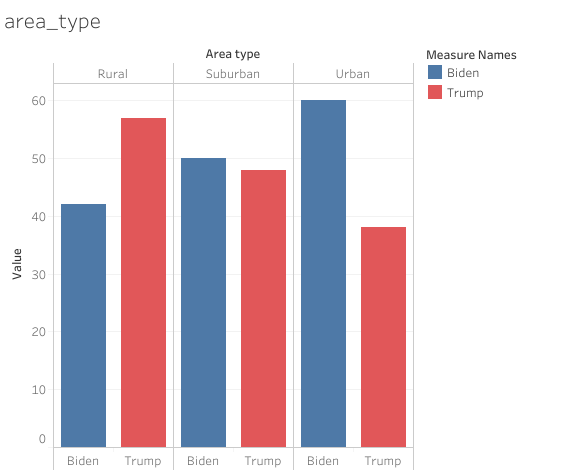
\includegraphics[width=0.6\textwidth]{figures/area_type.png}
        \caption{Tỷ lệ ủng hộ ứng cử viên theo khu vực sinh sống}
    \end{figure}


    \begin{figure}[h!]
        \centering
        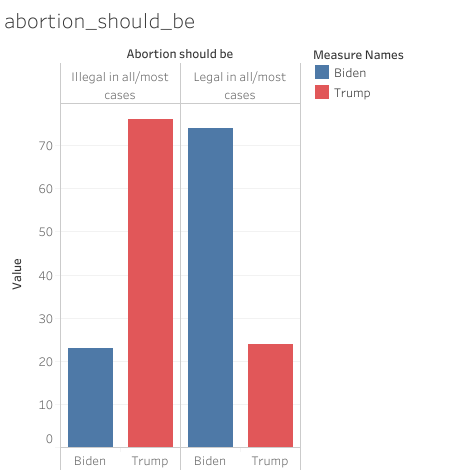
\includegraphics[width=0.6\textwidth]{figures/abortion_should_be.png}
        \caption{Tỷ lệ ủng hộ ứng cử viên theo quan điểm về nạo phá thai}
    \end{figure}

    Các ứng cử viên có quan điểm trái ngược nhau về vấn đề này, với Joe Biden và Đảng Dân chủ ủng hộ việc bảo vệ quyền phá thai và tiếp cận các dịch vụ phá thai an toàn và hợp pháp, trong khi Donald Trump và Đảng Cộng hòa tìm cách hạn chế hoặc cấm phá thai. 
    Kết quả của cuộc bầu cử có ý nghĩa quan trọng đối với tương lai của chính sách phá thai ở Hoa Kỳ.


    Trong thời gian chuẩn bị cho Cuộc bầu cử Tổng thống Hoa Kỳ năm 2020, các phương tiện truyền thông lớn, bao gồm các mạng truyền hình và tổ chức tin tức, đã tiến hành nhiều cuộc thăm dò và khảo sát để dự đoán kết quả của cuộc bầu cử. 
    Những dự báo này dựa trên nhiều yếu tố, bao gồm các kiểu bỏ phiếu trước đây, các xu hướng chính trị và xã hội hiện tại, cũng như kết quả của các cuộc thăm dò dư luận và khảo sát những cử tri có khả năng bầu cử. 
    Cuối cùng, phần lớn các phương tiện truyền thông lớn dự đoán rằng Joe Biden sẽ thắng cử, điều này đã được xác nhận khi ông nhận được 306 phiếu đại cử tri so với 232 phiếu đại cử tri của Donald Trump. 
    Tuy nhiên, cuộc bầu cử được nhiều người coi là có tính cạnh tranh cao, với cả hai chiến dịch tranh cử khắc nghiệp về kết quả và kết quả cuối cùng không được xác định cho đến vài ngày sau ngày bầu cử.

    \begin{figure}[h!]
        \centering
        \begin{subfigure}[b]{\textwidth}
            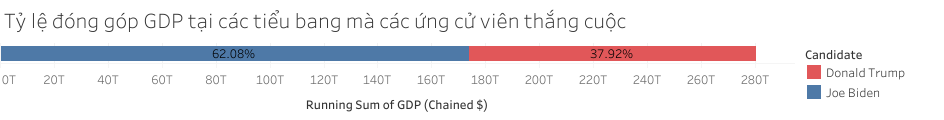
\includegraphics[width=0.9\textwidth]{State_Percentage_GDP_Candidate.png}
            \caption{Tỷ lệ đóng góp GDP tại các tiểu bang mà các ứng cử viên thắng}
        \end{subfigure}
        \vfill
        \begin{subfigure}[b]{\linewidth}
            \includegraphics[width=0.9\linewidth]{State_Percentage_Population_Candidate.png}
            \caption{Tỷ lệ đóng góp dân số tại các tiểu bang mà các ứng cử viên thắng}
        \end{subfigure}
        \vfill
        \begin{subfigure}[b]{\textwidth}
            \includegraphics[width=0.9\linewidth]{County_Total_Percentage_Candidate_Win.png}
            \caption{Tỷ lệ thắng trên các hạt của từng ứng cử viên}
        \end{subfigure}
        \vfill
        \begin{subfigure}[b]{\textwidth}
            \includegraphics[width=0.9\linewidth]{County_Percentage_Population_Candidate.png}
            \caption{Tỷ lệ đóng góp dân số tại các hạt mà các ứng cử viên thắng}
        \end{subfigure}
        \caption{So sánh quy mô dân số và kinh tế tại các bang, hạt các ứng cử viên chiến thắng}
    \end{figure}

    \section{Phân tích các yếu tố trong nhân khẩu học}

    Dữ liệu ta sử dụng là 

    Ta sẽ phân tích các yếu tố nhân khẩu học dựa trên xây dựng trên các mô hình học máy.
    Mục tiêu chính của ta khi xây dựng một mô hình học máy để dự đoán các ứng viên đảng Cộng hòa có thể thắng cuộc ở hạt nào mà ta sẽ sử dụng mô hình học máy để xem nhân tố nhân khẩu học nào quan trọng ảnh hưởng đến kết quả chiến thắng tại các hạt.
    Ta sẽ xây dựng hai loại mô hình học máy. 
    Loại mô hình thứ nhất là mô hình hồi quy dự đoán tỷ lệ phiếu bầu của ứng viên đảng Cộng hòa tại một hạt.
    Loại mô hình thứ hai là mô hình phân loại dự đoán liệu ứng viên đảng Cộng hòa có thắng tại hạt đó hay không.

    Ở loại mô hình thứ nhất, ta sử dụng 3 mô hình, mô hình thứ nhất là mô hình đơn giản, ta chỉ tính trung bình tỷ lệ được bỏ phiếu tại tất cả các hạt.
    Mô hình thứ hai là sử dụng mô hình hồi quy tuyến tính, mô hình thứ ba là mô hình XGBoost.





    \newpage
    \addcontentsline{toc}{section}{TÀI LIỆU THAM KHẢO}
    \printbibliography[title={TÀI LIỆU THAM KHẢO}]
\end{document}